\documentclass{scrartcl}
\usepackage[utf8]{inputenc}
\usepackage[spanish,es-tabla]{babel}	% Paquete de idiomas 'babel':
						%
						% 	Idioma: 'spanish'
						%	Opciones:
						%		es-tabla: sustituye la palabra 'cuadro' por 'tabla'.

\usepackage{amsmath,amsfonts,amsthm}
\usepackage{txfonts}	% Fuente Times
\renewcommand{\sectfont}{\rmfamily \bfseries} %cabeceras y titulos con estilo roman, negrita.


\usepackage{booktabs}	% Permite construir tablas de alta calidad.

\usepackage{xspace}

\usepackage[thinspace,mediumqspace,squaren]{SIunits}	% Sistema Internacional de unidades.
	\newcommand{\micras}{\micro\meter\xspace}
	\newcommand{\mm}{\milli\meter\xspace}
	\newcommand{\cm}{\centi\meter\xspace}
	\newcommand{\nm}{\nano\meter\xspace}

	\newcommand{\Exp}[1]{\cdot\power{10}{#1}}
	\newcommand{\vect}[1]{\mathbf{#1}}

%% TikZ %%
%
\usepackage{tikz}
\usepackage{pgfplots}
\pgfplotsset{compat=1.3}


\usepackage{float}
\newfloat{grafica}{htbp}{log}
\floatname{grafica}{Gráfica}
\usepackage{hyperref}

%% TikZ %%
%
\usepackage{tikz}


\renewcommand{\thesubsection}{\thesection.\alph{subsection}}
\usepackage[makeroom]{cancel}

\title{Base de datos en MySQL}
\subtitle{Sistemas de Gestión de Datos Científicos}
\author{Ignacio Suárez Andrés}
\date{4 de marzo de 2015}

\begin{document}
\maketitle

\section{Descripción del problema}
El objetivo es crear una base de datos de Pokémon de la que se pueda extraer información con resultados similares a los de la web \href{http://bulbapedia.bulbagarden.net/wiki/Main_Page}{Bulbapedia}, de donde se han extraído gran parte de los datos.\par
La base de datos contiene información asociada a una selección de especies de Pokémon, tipos elementales, grupos de compatibilidad para la reproducción, habilidades y movimientos que los Pokémon aprenden al ganar experiencia y subir de nivel. Se han establecido las relaciones existentes entre los datos anteriores, que están además descritos por los atributos más representativos.\par


\section{Funcionamiento de la base de datos}
La base de datos describe una serie de relaciones $N\rightarrow N$ mediante tablas intermedias con Foreign Keys asociadas a las tablas cuya información combinan. Las Foreign Keys se utilizan también como método de controlar que un atributo tome valores únicamente dentro de un conjunto permitido. Estas relaciones se pueden ver gráficamente en el diagrama EER en la figura \ref{fig:diagrama}. Con esta construcción, se pueden extraer de manera compacta conjuntos de información que requiere estar almacenada en varias tablas, sirviendo de ejemplo la consulta de la figura \ref{fig:helix}.\par

Se han incluido también funciones sencillas que involucran sumas de datos de tipo numérico, cuyos resultados pueden ser mostrados en una consulta como un atributo más. El uso de una de ellas se muestra en la consulta de la figura \ref{fig:rain}.\par
\begin{figure}[ht]
\centering
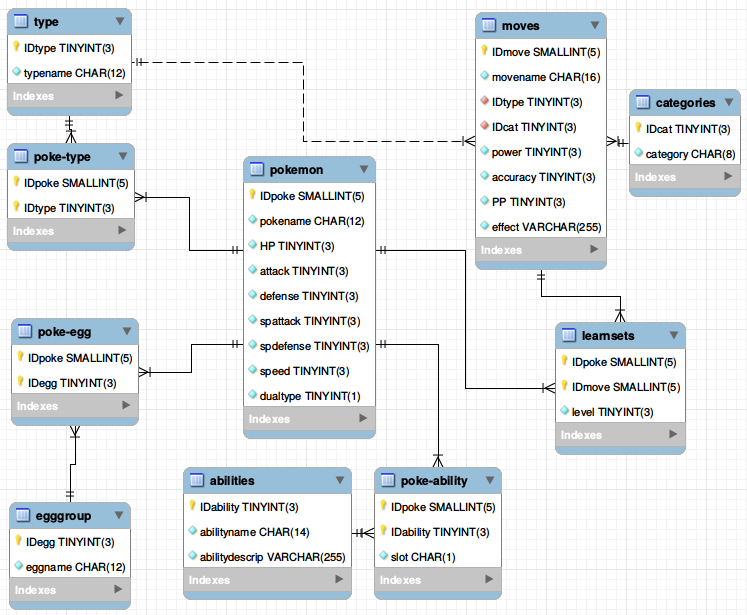
\includegraphics[scale=0.6]{diagramadb}
\caption{Diagrama EER de la base de datos de Pokémon.}
\label{fig:diagrama}
\end{figure}

\begin{figure}[ht]
\centering
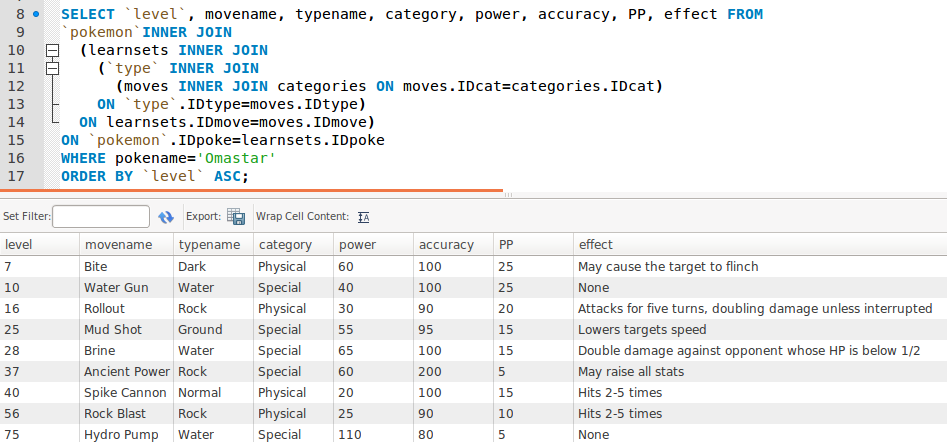
\includegraphics[scale=0.45]{consultahelix}
\caption{Consulta: Lista de movimientos que aprende Omastar, en qué nivel los aprende, tipo, categoría y demás atributos que caracterizan al movimiento.}
\label{fig:helix}
\end{figure}

\begin{figure}[ht]
\centering
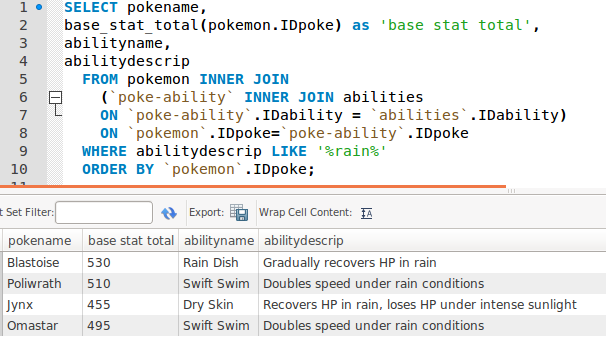
\includegraphics[scale=0.6]{consultarain}
\caption{Consulta: Se buscan los Pokémon que puedan tener una habilidad que les permita aprovecharse de la condición de lluvia. Se pide además un número que da una idea aproximada de la fuerza del Pokémon, calculado a partir de la suma de varios atributos.}
\label{fig:rain}
\end{figure}

\clearpage
\section{Posibles mejoras}
Las principales mejoras que se pueden proponer implican el uso de disparadores para suplir la falta de la orden CHECK en MySQL. Concretamente, se podrían limitar los valores aceptados en el atributo \texttt{level} de la tabla \texttt{learnsets} entre 1 y 100 ya que, salvo fallos del juego, un Pokémon no puede alcanzar un nivel fuera de ese rango. De modo similar, se podría forzar que no haya más de tres categorías de movimientos o posibles slots de habilidades, así como que un Pokémon no pueda estar asociado a más de dos grupos huevo.\par

\end{document}